\documentclass{standalone}
\usepackage{tikz}
\usetikzlibrary{positioning,fit,arrows.meta,backgrounds}

\tikzset{
    module/.style={%
        draw, rounded corners,
        minimum width=#1,
        minimum height=7mm,
        font=\sffamily
        },
    module/.default=2cm,
    >=LaTeX
}

\begin{document}
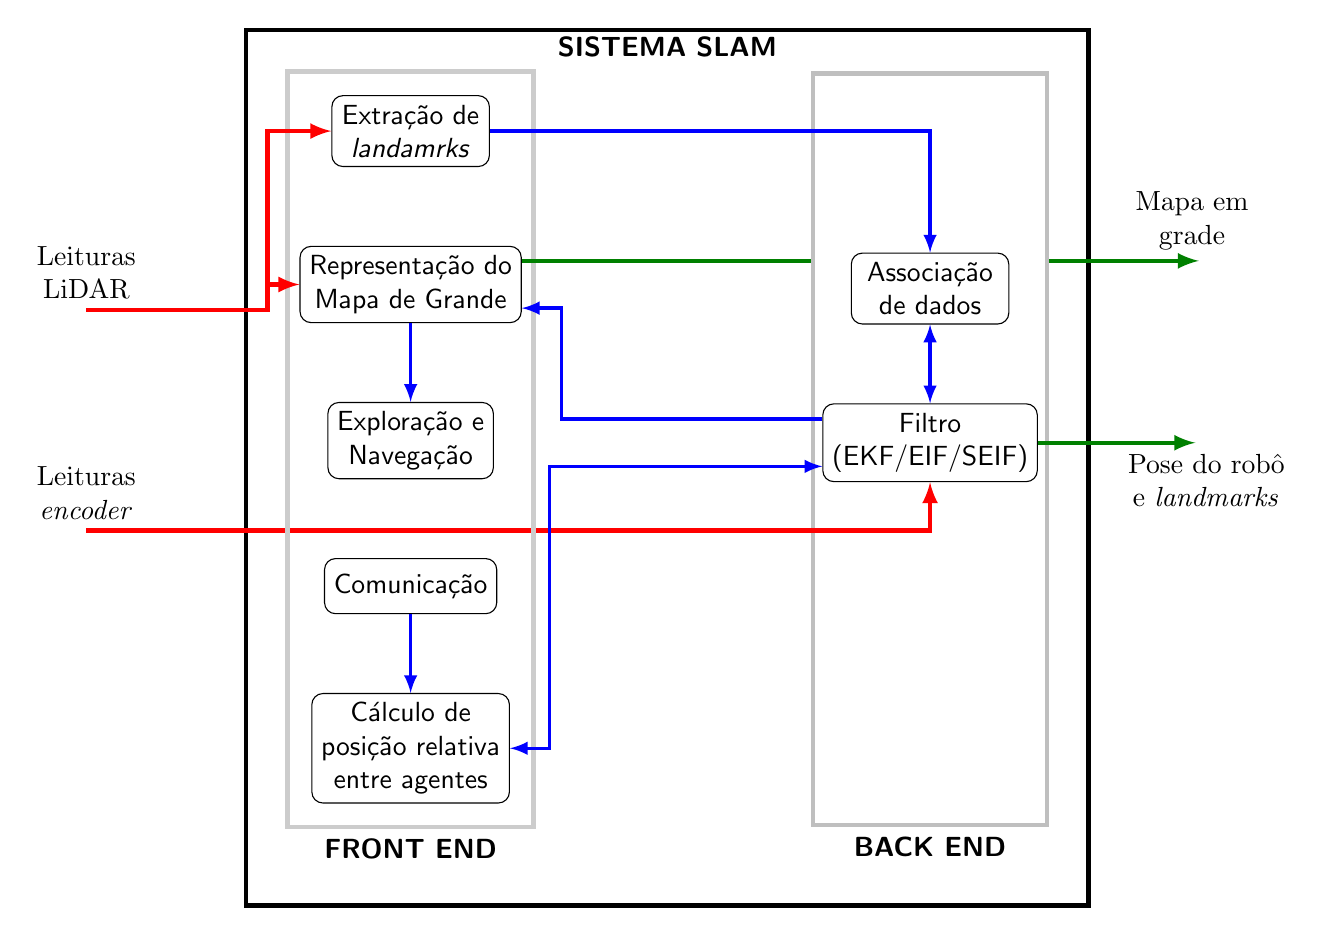
\begin{tikzpicture}

\node[module, align=center] (F1) {Extração de\\\textit{landamrks}};

\node[module, align=center, below=of F1] (F4) {Representação do\\Mapa de Grande};

\node[module, align=center, below=of F4] (F5) {Exploração e\\Navegação};

\node[module, below=of F5] (F2) {Comunicação};

\node[module, below=of F2, align=center] (F3) {Cálculo de\\posição relativa\\entre agentes};

\node[fit=(F1) (F2) (F3), draw=black!20, ultra thick, inner sep=3mm] (Frontend) {};


\node[anchor=north, font=\sffamily\bfseries] at (Frontend.south) {FRONT END};

\node[module, right=4cm of {F1 -| Frontend.east}, align=center, yshift=-2cm] (B1) {
 Associação\\de dados
};

\node[module, below=of B1, align=center] (B2) { Filtro\\(EKF/EIF/SEIF)};

\node[fit={(B1) (B1|-Frontend.north) (B1|-Frontend.south)
  (B2)}, draw=black!25, ultra thick, inner ysep=-\pgflinewidth] (Backend) {};

\node[anchor=north, font=\sffamily\bfseries] (BackendText) at (Backend.south) {BACK END};


\node[fit={(Frontend) (Backend) (BackendText)}, draw, ultra thick, inner sep=5mm] (System) {};

\node[anchor=north, font=\sffamily\bfseries] at (System.north) {SISTEMA SLAM};

\draw[-latex, ultra thick, red] ([shift={(-2cm,-0.8cm)}]System.west) node[anchor=south, align=center] {\color{black}Leituras\\\color{black}\textit{encoder}} -- ([yshift=-0.8cm]System.west -| B2.south) -- (B2);

\node[fit=(F1) (F2) (F3), draw=black!20, ultra thick, inner sep=3mm] (Frontend) {};

\draw[-latex, ultra thick, red] ([shift={(-2cm,2cm)}]System.west) node[anchor=south, align=center] {\color{black}Leituras\\\color{black}LiDAR} -- ([shift={(3mm,2cm)}]System.west) -- ([xshift=3mm]System.west |- F1.west) -- (F1);
\draw[-latex, ultra thick, red] ([shift={(3mm,2cm)}]System.west) -- ([shift={(3mm,0cm)}]System.west |- F4.west) -- (F4.west);

\draw[latex-latex, very thick, blue] (F3.east) -- node {} ++(.5,0) |- ([shift={(0,-3mm)}]B2.west);

\draw[latex-latex, very thick, blue] (B1) -- (B2);

\draw[-latex, very thick, blue] (F1) -- (F1.east -| B1.north) -- (B1);

\draw[latex-, very thick, blue] ([yshift=-3mm]F4.east) -- node {} ++(.5,0) |- ([shift={(0,3mm)}]B2.west);

\path[-latex, very thick, blue] (F2) edge (F3);

\draw[-latex, draw=green!50!black, ultra thick, align=center] (B2.east) -- node[anchor=north west] (output) {Pose do robô\\e \textit{landmarks}} ++(right:2);

\draw[draw=green!50!black, ultra thick] ([yshift=3mm]F4.east) -- ([yshift=3mm]F4.east -| Backend.west);

\draw[-latex, draw=green!50!black, ultra thick] ([yshift=3mm]F4.east -| Backend.east) -- node[anchor=south west, align=center] {Mapa em\\grade} ++(right:1.9cm);

\draw[-latex, very thick, blue] (F4) -- (F5);

\end{tikzpicture}
\end{document}